\documentclass{standalone}
%
\usepackage{tikz}
%
\usepackage{tkz-euclide}
%
\usepackage{xcolor}
\definecolor{earth}{HTML}{0089FA}
\definecolor{dida}{HTML}{FFDE00}
\definecolor{title}{HTML}{FBA706}
%
\usepackage{fontspec}
\setmainfont{Open Dyslexic}
%
\title{La notte di San Lorenzo}
\begin{document}
	\tikzset{
		partial ellipse/.style args = {#1:#2:#3}{insert path={+ (#1:#3) arc (#1:#2:#3)}},
	}
	\begin{tikzpicture}
		\draw [use as bounding box,color=white] (0,15.5) -| (30,15.5) |- (30,-58) -| (0,-58);
		%title
		\draw [black,ultra thick,fill=title] (-1,7) rectangle (31,15);
		\node (example-textwidth-2) [right, align=center, text width=30cm, color=black, font=\fontsize{90pt}{91pt}\selectfont] at (0,11) {La notte di San Lorenzo};
		%
		\begin{scope}[shift={(0,-2)}]
			\node at (21,0) {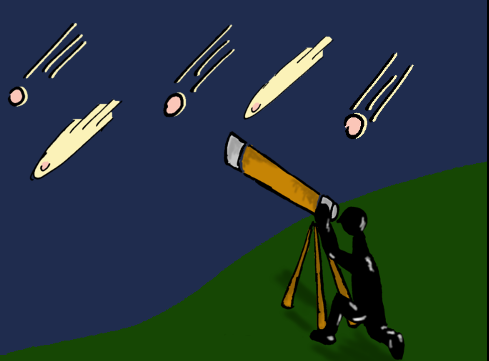
\includegraphics[width=14cm]{astrofilo}};
			\draw [ultra thick] (14,5.2) rectangle (28,-5.2);
			\draw [ultra thick, fill=dida] (1,-8) rectangle (14,8);
			\node (example-textwidth-2) [right, align=left, text width=12cm, color=black, font=\fontsize{23pt}{24pt}\selectfont] at (1.5,0) {La notte di san Lorenzo è tradizionalmente associata al passaggio dello sciame meteorico delle Perseidi, fenomeno popolarmente ed erroneamente chiamato stelle cadenti ma anche poeticamente lacrime di San Lorenzo, considerato evocativo dei carboni ardenti su cui il santo fu martirizzato. In effetti, in quei giorni, l'atmosfera terrestre è attraversata da un numero di piccole meteore molto più alto del normale.};
		\end{scope}
		%
		\begin{scope}[shift={(0,-20)}]
			\node at (8.5,0) {
\includegraphics[width=14cm]{swift}};
			%dida
			\draw [ultra thick] (1.5,9) rectangle (15.5,-9);
			\draw [ultra thick, fill=earth!50!white] (5.5,-8.5) rectangle (11.5,-9.5);
			\node (example-textwidth-2) [right, align=center, text width=11.5cm, color=black, font=\fontsize{23pt}{24pt}\selectfont] at (2.7,-9) {Lewis Swift};
			\draw [ultra thick, fill=dida] (16.5,11) rectangle (29,-13);
			\node (example-textwidth-2) [right, align=left, text width=11.5cm, color=black, font=\fontsize{23pt}{24pt}\selectfont] at (17,-1) {Le Perseidi sono uno sciame meteorico che la Terra si trova ad attraversare durante il periodo estivo nel percorrere la sua orbita intorno al Sole. La pioggia meteorica si manifesta dalla fine di luglio fino oltre il 20 agosto e il picco di visibilità è concentrato attorno al 12 agosto, con una media di circa un centinaio di scie luminose osservabili ad occhio nudo ogni ora.\\La cometa che ha dato origine a questo sciame è la Swift-Tuttle, che ha un nucleo di circa 10 km.\\E' stata scoperta indipendentemente da Lewis Swift il 16 luglio del 1862 e da Horace Parnell Tuttle il successivo 19 luglio.};
		\end{scope}
		%
		\begin{scope}[shift={(0,-40)}]
			\node at (22,0) {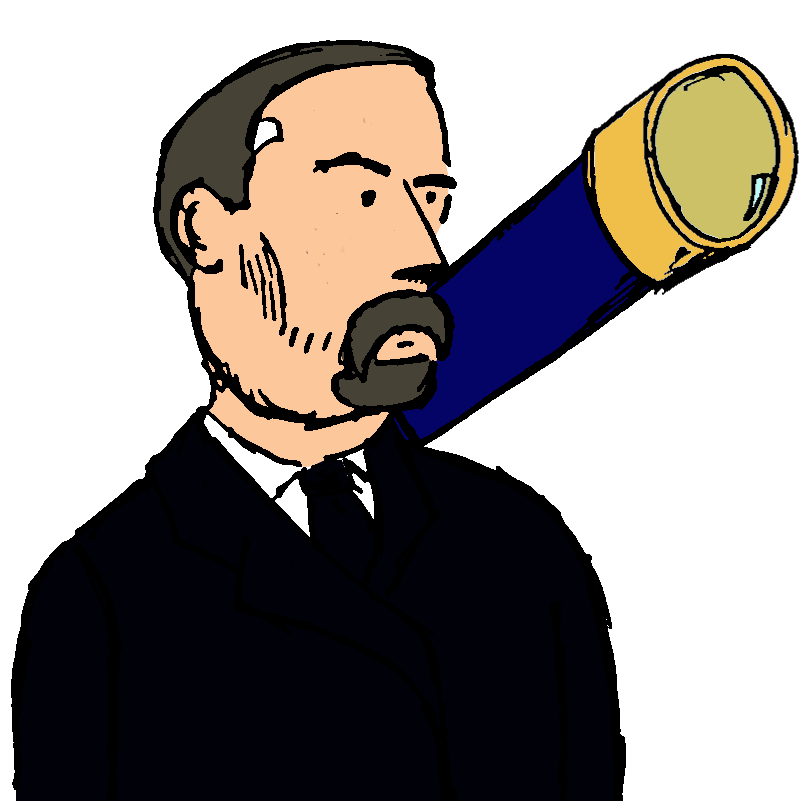
\includegraphics[width=13cm]{schiaparelli}};
			\draw [ultra thick] (15.5,6.3) rectangle (28.5,-6.3);
			\draw [ultra thick, fill=earth!50!white] (17,-6.8) rectangle (27,-5.8);
			\node (example-textwidth-2) [right, align=center, text width=11.5cm, color=black, font=\fontsize{23pt}{24pt}\selectfont] at (16.1,-6.3) {Giovanni Schiaparelli};
			%
			\draw [ultra thick, fill=dida] (1,-0.5) rectangle (18,6.5);
			\node (example-textwidth-2) [right, align=left, text width=16cm, color=black, font=\fontsize{23pt}{24pt}\selectfont] at (1.5,3) {Il legame con lo sciame meteorico delle Perseidi fu scoperto da Giovanni Schiaparelli nel 1866, a seguito del passaggio al perielio della cometa del 1862, come riportato in un suo scambio epistolare con Padre Angelo Secchi.};
		\end{scope}
		%
		\begin{scope}[shift={(0,-46)}]
			\node at (8.5,0) {
\includegraphics[width=10cm]{jan_oort}};
			\draw [ultra thick, fill=dida] (0.5,-4.5) rectangle (29,-9.5);
			\node (example-textwidth-2) [right, align=left, text width=28cm, color=black, font=\fontsize{23pt}{24pt}\selectfont] at (1,-7) {Si ritiene che le comete, corpi celesti simili agli asteroidi ma composti di ghiaccio, siano originarie della nube di Oort, una distribuzione sferica di oggetti che costituisce il confine del Sistema Solare, la cui esistenza è stata ipotizzata dall'astronomo olandese Jan Oort.};
		\end{scope}
		%
		\begin{scope}[shift={(0,-56.7)}]
			\node at (27,0) () {
\includegraphics[width=3.7cm]{licenza}};
			\node (example-textwidth-2) [right, align=left, text width=23.5cm, color=black, font=\fontsize{14pt}{15pt}\selectfont] at (1.5,-0.1) {Testo estratto dalle voci della Wikipedia in lingua italiana: San Lorenzo (paragrafo "Notte di San Lorenzo"), Perseidi, Cometa Swift-Tuttle, Cometa.\\
			Illustrazioni: @ulaulaman - Gianluigi Filippelli};
		\end{scope}
	\end{tikzpicture}
%
\end{document}